\section{Testing for significant edges in incoherent signal subnetworks}
\label{sec:ch9:ssn_incoherent}

For the remainder of this section, we will revisit the problem that we covered in Section \ref{sec:ch5:multicovar}. From Example \ref{box:ch5:multicovar:ssn_ex}, we had $M=200$ networks collected from either earthlings ($y_m = 0$) or astronauts ($y_m = 1$). The nodes of these networks represented different areas of the brain, sight (SI), language (L), hearing/emotional expression (H/E), thinking/movement (T/M), and basic survival functions (BS). Edges represented whether pairs of nodes could pass information to one another. Over the course of $500,000$ years, the brains of astronauts adapted to the evolutionary pressures in their new environment, and the node responsible for sight relates to the other nodes in the network differently. 

The way in which we captured this disparity was via the $SSN$ model, in which the probability matrix for each edge depended on (1) which class the network was in, and (2) whether the edge is in the signal subnetwork (or not). For edges in the signal subnetwork, the probability of that edge existing for a given individual $m$ depended on the class of that individual. To start this section off, we will begin by simulating some data which we can work with. We will have $M=200$ people, and each person will be an earthling (with probability $\pi_0 = 0.55$) or an alien (with probability $\pi_1 = 0.45$):

\begin{lstlisting}[style=python]
import numpy as np

pi_astronaut = 0.45
pi_earthling = 0.55
M = 200

# roll a 2-sided die 200 times, with probability 0.45 of landing on side 2 (astronaut)
# and probability 0.55 of landing on side 1 (earthling)
classnames = ["Earthling", "Earthling"]
ys = np.random.choice(2, p=[pi_earthling, pi_astronaut], size=M)
print("Number of individuals who are earthlings: {:d}".format((ys == 0).sum()))
print("Number of individuals who are astronauts: {:d}".format((ys == 1).sum()))
\end{lstlisting}

Next, we construct the probability matrices for each class. The probabilities for edges in which a node is in the sight area are higher for the astronauts than for the earthlings:

\begin{lstlisting}[style=python]
n = 5
P_earthling = 0.3*np.ones((n, n))

nodenames = [
    "SI", "L", "H/E", 
    "T/M", "BS"
]

signal_subnetwork = np.zeros((n, n), dtype=bool)
signal_subnetwork[1:n, 0] = True
signal_subnetwork[0, 1:n] = True
P_astronaut = np.copy(P_earthling)

# probabilities for signal edges are higher in astronauts than earthlings
P_astronaut[signal_subnetwork] = np.tile(np.linspace(0.4, 0.9, num=4), 2)
\end{lstlisting}

Back in Figure \ref{fig:ch5:ssg_pmtxs} and \ref{fig:ch5:ssg_ssn}, we saw that the probability matrices differed between the astronauts and the earthlings for all edges which included a node from the sight area (SI). These edges, we attributed, comprised the ``signal subnetwork'', in that the class-specific difference (the \textit{signal}) was different between them.

In Section \ref{sec:ch5:multicovar}, we saw how we could formulate the problem using the $SSN$ model, and Algorithm \ref{alg:ch5:ssn} gave us a procedure that we could use to generate samples of $SSN$ networks:


\begin{lstlisting}[style=python]
# the probability matrices for each class
Ps = [P_earthling, P_astronaut]

# sample networks with the indicated probability matrix
As = np.stack([sample_edges(Ps[y]) for y in ys], axis=2)
\end{lstlisting}

So, how do we actually use this model, in practice? Stated another way, given a collection of networks from multiple classes, how do we find the set of edges which differ most between the classes (and estimate the signal subnetwork), and how do we use this information to classify brain networks as earthling or astronaut?

To break these down explicitly, we have the following aims:

\begin{enumerate}
    \item We want to look at the edges which have a differing connection probability amongst our classes. This means that we only want to look at \textit{signal edges} which are in the \textit{signal subnetwork}, and we want to ignore edges which are not in the signal subnetwork. Edges which are not in the signal subnetwork are simply noise, since they have the same connection probability between the classes, and therefore are not useful for differentiating between the different classes.
    \item We want to be able to incorporate these signal and non-signal edges into a structured classifier, which predicts whether a network is from an earthling or astronaut.
    \item We want to be able to incorporate information about the network structure into our classifier.
\end{enumerate}

\subsection{Using \textit{edge importances} to estimate the signal subnetwork}

Let's start by thinking about the first aim: differentiating which edges carry signal (they are in the signal subnetwork) given a collection of networks with class labels. 

To do this, we will return to the Fisher's exact test, which you first learned about in Section \ref{sec:ch7:testing:twosample} and revisited in Table \ref{tab:ch8:twosampl_sbm:cont}. 
As it turns out, we can adapt this test for our situation here too.

For a single edge, what we want to do is test whether $H_A: p_{ij}^{(0)} \neq p_{ij}^{(1)}$, against the null hypothesis that $H_0: p_{ij}^{(0)} = p_{ij}^{(1)}$. Stated another way, we want to differentiate whether or not the probabilities for that edge differ between earthling and astronaut brain networks. The key property of Fisher's exact test that makes it desirable for us is that, in a sense, when there is more evidence to support $H_A$, the $p$-value will tend to be smaller (we would tend to reject the null hypothesis). When there is more evidence to support $H_0$, the $p$-value will tend to be larger (we would not have evidence to reject the null hypothesis). We will exploit this feature in our design of a classifier for aliens versus earthlings. For each edge $(i, j)$, we construct the table shown in Table \ref{tab:ch9:ssn:fet}.

\begin{table}[]
    \centering
    \begin{tabular}{p{4cm} | p{3cm} | p{3cm}}
         & Earthlings & Astronauts  \\
        \hline
         Number of networks where edge $(i, j)$ exists & $a$ & $b$ \\
         Number of networks where edge $(i, j)$ does not exist & $c$ & $d$ \\
         \hline
    \end{tabular}
    \caption{A contingency table for edge existences/non-existences between each of the two classes.}
    \label{tab:ch9:ssn:fet}
\end{table}

Which we can do in python as follows, for the edge from the sight area to the basic survival area:

\begin{lstlisting}[style=python]
def generate_table(As, ys, i, j):
    """
    A function to generate a contingency table for a given edge.
    """
    # count the number of earthlings with edge i,j
    a = As[i,j,ys == 0].sum()
    # count the number of astronauts with edge i,j
    b = As[i,j,ys == 1].sum()

    c = len(As[i,j,ys == 0]) - a
    d = len(As[i,j,ys == 1]) - b
    
    edge_tab = np.array([[a, b], [c, d]])
    return edge_tab

# edge (0, 4) corresponds to SI to BS
edge_tab = generate_table(As, ys, 0, 4)
print(edge_tab)
\end{lstlisting}

Next, we compute the Fisher's exact test $p$-value, using \texttt{scipy}:

\begin{lstlisting}[style=python]
from scipy.stats import fisher_exact

_, pval = fisher_exact(edge_tab)
print("p-value: {:.4f}".format(pval))
\end{lstlisting}

That the $p$-value for this edge is small tells us that we have evidence to reject the null hypothesis here in favor of the alternative hypothesis; that the edge from SI to BS in fact shows a disparity between earthlings and astronauts. Why is this a big deal?

Let's see what happens when we repeat this process for a non-signal edge. We arbitrarily choose the edge between H/E and L areas, corresponding to $i=2$ (H/E) and $j=1$ (L):

\begin{lstlisting}[style=python]
_, pval = fisher_exact(generate_table(As, ys, 2, 1))
print("p-value: {:.4f}".format(pval))
\end{lstlisting}

The interpretation of this test is that we do not have evidence to reject the null hypothesis that the edge from L to H/E areas has the same probability in earthlings and astronauts. 

For signal edges the $p$-value will, by construction, generally (but not always) be smaller than the $p$-value in a non-signal edge. We could certainly get samples of data where this is not the case, analogous to the idea that we could flip a fair coin (with equal probability of seeing heads and tails) $10$ times and obtain all $10$ outcomes being heads. 

Despite this hurdle, we can use the Fisher's exact test to quantify how ``important'' an edge is for differentiating the two classes, also known as an \textit{edge importance} statistic. In this case, an edge importance statistic with a higher value denotes that the edge is more important for the task at hand, which here is differentiating the two classes. We will do this by ranking the $p$-values from largest (lower ranks) to smallest (higher ranks), where the edges with the higher ranks are more important for differentiating the classes.

Since the networks are loopless, we can ignore the diagonal, and since the networks are undirected, we can compute the $p$-values for a single triangle and then symmetrize the resulting fisher $p$-value matrix. Then, we rank the edges, from largest to smallest, in terms of the $p$-values using \texttt{scipy}. Note that the \texttt{scipy} function \texttt{rankdata()} natively ranks values from smallest to largest, so to rank positive data from largest to smallest, we can first negate the matrix of Fisher test $p$-values:

\begin{lstlisting}[style=python]
from graspologic.utils import symmetrize
from scipy.stats import rankdata

fisher_mtx = np.empty((n, n))
fisher_mtx[:] = np.nan

for i in range(0, n):
    for j in range(i+1, n):
        fisher_mtx[i, j] = fisher_exact(generate_table(As, ys, i, j))[1]
fisher_mtx = symmetrize(fisher_mtx, method="triu")
# use rankdata on -fisher_mtx, to rank from largest p-value to smallest p-value
edge_imp = rankdata(-fisher_mtx, method="dense", nan_policy="omit").reshape(fisher_mtx.shape)
np.fill_diagonal(edge_imp, 0)
\end{lstlisting}

The resulting edge importance matrix is shown in Figure \ref{fig:ch9:ssn:ssn_inco_edgeimp}(B) along with the signal subnetwork in Figure \ref{fig:ch9:ssn:ssn_inco_edgeimp}(A). Notice that edges which are in the signal subnetwork tend to have higher edge importances.

\begin{figure}[h]
    \centering
    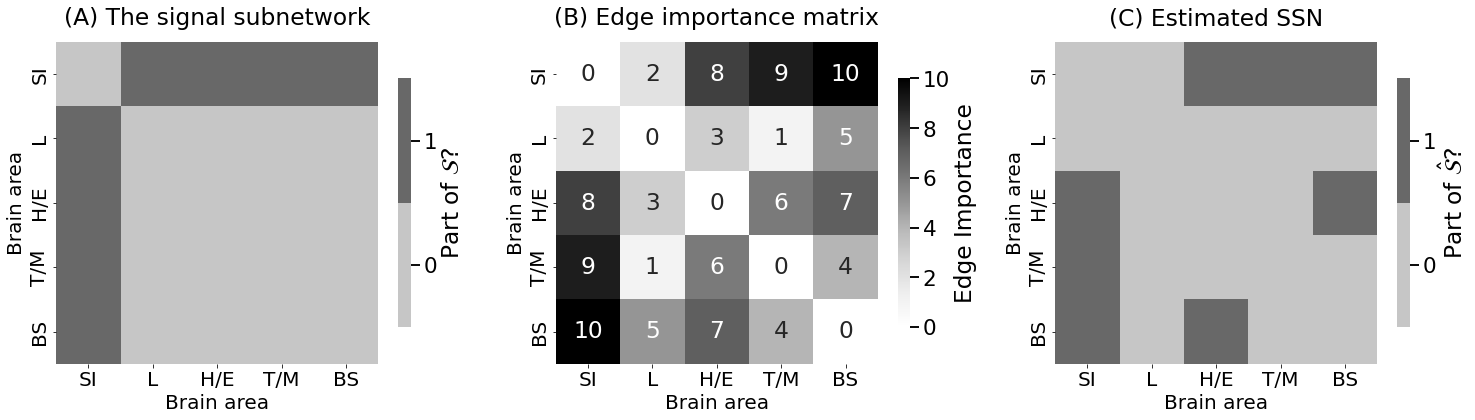
\includegraphics[width=\linewidth]{applications/ch9/Images/ssn_inco_edgeimp.png}
    \caption[Edge importances for incoherent signal subnetworks]{\textbf{(A)} the signal subnetwork for the earthling and astronauts, \textbf{(B)} the edge importances for differentiating earthlings from astronauts.}
    \label{fig:ch9:ssn:ssn_inco_edgeimp}
\end{figure}

We can use this to estimate what is known as an \textit{incoherent} signal subnetwork by simply finding the edges corresponding to the $K$ highest edge importances.

We can implement this process using \texttt{graspologic} to estimate the signal subnetwork like we do below, where we estimate a signal subnetwork with $8$ edges:

\begin{lstlisting}[style=python]
from graspologic.subgraph import SignalSubgraph

K = 8  # the number of edges in the subgraph
ssn_est = SignalSubgraph()
ssn_est.fit_transform(As, labels=ys, constraints=K);

sn_est = np.zeros((n,n))  # initialize empty matrix
sn_est[sgest.sigsub_] = 1
\end{lstlisting}

The estimated signal subnetwork $\hat{\mathcal S}$ with $K=8$ edges is shown in Figure \ref{fig:ch9:ssn:ssn_inco_edgeimp}(C). Notice that when we ran the simulation, our results were imperfect: while $6$ of $8$ of the estimated signal edges are in the true signal subnetwork, we got $2$ edges incorrect. In the event that the difference in probabilities between the different classes is large, as was the case for the $6$ edges we got correct, this procedure will tend to reach reasonably stable conclusions, in that our estimates will faithfully reflect the underlying signal subnetwork. However, when the difference in probabilities between the different classes is smaller (such as for the SI and L edge, which we got wrong) we might estimate the signal subnetwork incorrectly for a given number of networks $M$.

\subsection{Building a classifier using the estimated signal subnetwork}

We can use the estimated signal subnetwork that we have constructed to devise a classifier. The objective of a classifier is to take new samples of data (which in this case are networks), and assign them to the class which they are most likely from. How do we determine this given an estimated signal subnetwork $\hat{\mathcal S}$?

In this case, since our networks (and hence, the signal edges) are binary, a logical place to start is known as a bernoulli Naive Bayes classifier. For details on the Naive Bayes classifier, check out Appendix \ref{app:ch14:bayes} and the original paper for signal subnetworks \cite{Vogelstein2013Jul}.

\subsubsection*{Network classification}

When the features of our data are binary (such as the adjacency matrix of a network), a reasonable Naive Bayes classifier to use would be the \texttt{BernoulliNB} classifier from \texttt{sklearn}. Our estimated signal subnetwork $\hat{\mathcal S}$ is returned to us by \texttt{graspologic} in the form of a \texttt{[2 x K]} matrix, where $K$ is the number of edges in the signal subnetwork. The first row is the row index of the entry of the signal subnetwork, and the second row is the column index of the entry in the signal subnetwork. We need to coerce this into an \texttt{[M x K]} matrix which we will call the data matrix $D$, where $M$ is the total numberof networks, and $K$ is the number of edges in the signal subnetwork. Each entry of this matrix $d_{mk}$ will represent the adjacency matrix value of the $m^{th}$ individual for the $k^{th}$ element of the signal subnetwork. We can do this as follows:

\begin{lstlisting}[style=python]
D = As[ssn_est.sigsub_[0], ssn_est.sigsub_[1],:].T
\end{lstlisting}

Next, we create a Naive Bayes classifier, and fit the classifier using the classes $\vec y$ for all of our samples:

\begin{lstlisting}[style=python]
from sklearn.naive_bayes import BernoulliNB

classifier = BernoulliNB()
# fit the classifier using the vector of classes for each sample
classifier.fit(D, ys)
\end{lstlisting}

To evaluate our classifier's performance, we will create $200$ new ``held-out'' networks that were not used for training, and assess the performance of our classifier using the classification accuracy. If $h_{\hat\theta}\left(A^{(m)}\right)$ is the predicted class (either earthling, $0$, or astronaut, $1$) for a new held-out sample $A^{(m)}$ for the Naive Bayes classifier after training with parameters $\hat\theta = (\hat {\mathcal S}, K)$, the classification accuracy for $M'$ held-out samples is:
\begin{align*}
    \frac{1}{M'}\sum_{m = 1}^{M'}\mathfrak 1\left\{h_\theta\left(A^{(m)}\right) = y_m\right\},
\end{align*}
which simply computes the average number of correct answers produced by our classifier. In machine learning, it is typically a bad idea to evaluate the performance of a model using the data upon which you trained it, as you can easily run the risk of overfitting.

Let's begin by generating our held-out samples:

\begin{lstlisting}[style=python]
# number of heldout samples
Mp = 200
y_heldout = np.random.choice(2, p=[pi_earthling, pi_astronaut], size=M)
# sample networks with the appropriate probability matrix
A_heldout = np.stack([sample_edges(Ps[y]) for y in y_heldout], axis=2)

# compute testing data on the estimated signal subnetwork
D_heldout = A_heldout[sgest.sigsub_[0], sgest.sigsub_[1],:].T

yhat_heldout = classifier.predict(D_heldout)

# classifier accuracy is the fraction of predictions that are correct
heldout_acc = np.mean(yhat_heldout == y_heldout)
print("Classifier Testing Accuracy: {:.3f}".format(heldout_acc))
\end{lstlisting}

You should end up with a classifier with a relatively high held-out accuracy; when we ran this through, we saw accuracies between $80\%$ and $90\%$. 

Let's put this all together with a single function, which will use the training data to estimate a signal subnetwork and train a Naive Bayes classifier, and will produce accuracies using a separate set of ``testing'' networks:

\begin{lstlisting}[style=python]
def train_and_eval_ssn(Atrain, ytrain, Atest, ytest, K):
    """
    A function which trains and tests an incoherent signal subnetwork
    classifier with K signal edges.
    """
    ssn_est = SignalSubgraph()
    ssn_est.fit_transform(Atrain, labels=ytrain, constraints=int(K));

    Dtrain = Atrain[ssn_est.sigsub_[0], ssn_est.sigsub_[1],:].T
    classifier = BernoulliNB()
    # fit the classifier using the vector of classes for each sample
    classifier.fit(Dtrain, ytrain)

    # compute testing data on the estimated signal subnetwork
    Dtest = Atest[ssn_est.sigsub_[0], ssn_est.sigsub_[1],:].T
    yhat_test = classifier.predict(Dtest)
    
    # classifier accuracy is the fraction of predictions that are correct
    return (np.mean(yhat_test == ytest), ssn_est, classifier)
\end{lstlisting}

\subsubsection*{Parameter selection for signal subnetworks}

A core question for our incoherent signal subnetwork is: how do we determine an appropriate number of signal edges to include in our estimated signal subnetwork?

Similar to other machine learning techniques, we use cross validation. \textit{Cross validation} is a procedure in which we split the dataset into a number of approximately equally sized splits (called \textit{folds}), and then we train a machine learning model using a subset of the folds (the \textit{training folds}). We then test the trained model on the excluded subset of the folds (the \textit{testing folds}). We use a trained machine learning model which maximizes accuracy on the testing folds, and break ties using other desirable heuristics (for instance, arbitrarily selecting the simplest trained model which achieves maximal accuracy). 

For network classification using signal subnetworks, we can estimate the optimal number of signal edges using the procedure described in Algorithm \ref{alg:ch9:ssn}.

\begin{algorithm}
\label{alg:ch9:ssn}
\caption{Estimating the number of signal edges using cross validation}
\KwData{A set of networks and class labels $\left(A^{(m)}, y_m\right)$, for $m = 1, \hdots, M$. \newline
$K'$ the maximum number of possible signal edges.\newline
$L$ the number of folds to use for cross validation.}
\KwResult{$K^*$ the optimal number of signal edges.}
\SetAlgoLined

Split the indexing set $\left\{1, \hdots, M\right\}$ into $L$ folds of approximately equal size at random.

\For{$k = 1, \hdots, K'$}{
    \For{$l = 1, \hdots, L$}{
        Let $n_l$ denote the number of samples in fold $l$.

        Let $\hat{\mathcal S}$ be the estimated signal subnetwork with $k$ signal edges, which is estimated using the networks from the training folds $l' \neq l$.

        Train a Naive Bayes classifier using the training folds to produce a network classifier $h_{\hat \theta}$, which takes networks and produces class predictions.

        Let $a_{k,l}$ be the testing accuracy using the testing fold $l$.
    }
    Let $a_k = \frac{1}{n}\sum_{l = 1}^L n_l a_{k, l}$ be the testing accuracy over all $L$ folds for $k$ signal edges.
}
Let $K^* = \text{argmax}_k a_k$ be the number of signal edges which maximizes the testing accuracy. If there are multiple numbers of signal edges which maximize the testing accuracy, break ties by choosing the smallest such number of signal edges.

\Return{$K^*$.}
\end{algorithm}

We will implement this strategy using $L = 20$ folds, and will consider signal subnetworks with sizes ranging from $2$ to $20$ signal edges in increments of $2$. The reason that we exclude to increments of $2$ here is that our networks are undirected, which means that edge $(i, j)$ and edge $(j, i)$ will contain identical information. Further, the reason that we consider a maximum of $20$ signal edges is that the networks are loopless, so there are a maximum of $20$ possible signal edges in the network.

We can implement $20$-fold cross validation using \texttt{sklearn} as indicated below. Note that this procedure might take between $5$ and $10$ minutes, even on the small networks that we have been working with so far:

\begin{lstlisting}[style=python]
from sklearn.model_selection import KFold
import pandas as pd

kf = KFold(n_splits=20, random_state=None)
xv_res = []
for l, (train_index, test_index) in enumerate(kf.split(range(0, M))):
    A_train, A_test = As[:,:,train_index], As[:,:,test_index]
    y_train, y_test = ys[train_index], ys[test_index]
    nl = len(test_index)
    
    for k in np.arange(2, 20, step=2):
        acc_kl = train_and_eval_ssn(A_train, y_train, A_test, y_test, k)
        xv_res.append({"Fold": l, "k": k, "nl": nl, "Accuracy": acc_kl})
xv_data = pd.DataFrame(xv_res)

def weighted_avg(group):
    acc = group['Accuracy']
    nl = group['nl']
    return (acc * nl).sum() / nl.sum()

xv_acc = xv_data.groupby(["k"]).apply(weighted_avg)
print(xv_acc)
\end{lstlisting}

Which with our data, produces the table shown in Table \ref{tab:ch9:ssn_fold}. You might see slightly different results due to the fact that the simulation data used for this section was produced randomly. In our simulation, we reach optimal average testing accuracy with $6$ signal edges.

\begin{table}
\centering
\begin{tabular}{c|c}
    Number of signal edges & Average testing accuracy  \\
    \hline
    2 & 0.820\\
    4 & 0.785\\
    \rowcolor{lightgray!40} 6 & 0.875\\
    8 & 0.850\\
    10 & 0.865\\
    12 & 0.865\\
    14 & 0.860\\
    16 & 0.850 \\
    18 & 0.850 \\
    \hline
\end{tabular}
\caption{The average testing accuracy as a function of the number of signal edges. With $6$ signal edges, the optimal average testing accuracy is achieved, indicated by the light gray row.}
\label{tab:ch9:ssn_fold}
\end{table}

Once we have computed the optimal number of signal edges using cross validation, we would then estimate a signal subnetwork and train a classifier using the full training data with the optimal number of signal edges, and evaluate our signal subnetwork and the resulting classifier using any remaining held-out data. 

Using our method that we developed above, we could do this as follows:

\begin{lstlisting}
acc, ssn_est, classifier_est = train_and_eval_ssn(As, ys, A_heldout, y_heldout, 6)
\end{lstlisting}
